$subject$=Физические основы компьютерных \\ и сетевых технологий
$teacher$=Лекции Зинчика А. А.
$date$=10.11.2025

Также, так как электрон движется вокруг ядра, то создается ток, а значит и магнитное поле. Следовательно, атом обладает магнитным моментом $P_m = \frac{q v r}{2}$

Тогда появляется такое соотношение $\vec P_m = \frac{q}{2m} \vec L$. Получаем, что $P_m = \frac{q \hbar}{2 m} \sqrt{l (l + 1)}$. Для электрона $\mu_{\text{Б}} = \frac{e \hbar}{2 m_e} = 9.23 \cdot 10^{-24}$ -- магнетон Бора

Тогда, если $L_z = m \hbar$, то $P_{mz} = m \mu_{\text{Б}}$

Физический смысл магнитного квантового числа проявляется только в том случае, если атом находится в магнитном поле

\mediumvspace

Существование орбитального и магнитного квантовых чисел дает еще большее разделение энергетических уровней:

\begin{center}
    \includegraphics[height=10cm]{physics3/images/physics3_energetic_levels}
\end{center}

\mediumvspace

В 1921 году были проведены опыты Штерна и Герлаха

В ходе опытов было показано, что пучок атомов серебра, пройденный через неоднородное магнитное поле, на экране проявляются в виде двух симметричных пятен. Дело в том, что у атома есть собственный магнитный момент, который влиял на сторону попадания: $\vec F = p_{mz} \frac{d\vec B}{dz}$

Поэтому для частицы вводят спин -- характеристику, описывающую собственный момент количества движения частицы, не связанный с её движением в пространстве. Спин принимает квантованные значения и может ориентироваться в магнитном поле лишь определённым образом

\mediumvspace

У электрона спин может быть равным $\frac{1}{2}$ или $-\frac{1}{2}$

Частицы, у которых спин полуцелый $\left(\frac{1}{2}, \frac{3}{2}, \dots\right)$, называют фермионами, а те, у которых спин целый $(0, 1, 2, \dots)$, -- бозонами

Собственный механический момент импульса электрона равен $L_s = \hbar \sqrt{s(s+1)} = \frac{\sqrt{3}}{2}\hbar$, а собственный магнитный момент $p_{m s} = \sqrt{3},\mu_{\text{Б}}$

\mediumvspace

В одной молекуле соединяются только атомы с электронами, имеющие разные спины. Это связано с тем, что два электрона, находящиеся в одной атомной орбитали, не могут иметь одинаковые квантовые числа -- такая закономерность называется запретом Паули

Внешнее магнитное поле выделяет направленность в пространстве, и спин электрона может иметь только две проекции на направление поля

Это означает, что для каждого набора квантовых чисел $n$, $l$ и $m$ на данной орбитали могут находиться не более двух электронов, причём с противоположными спинами

Поэтому инертные газы ($\mathrm{He}$, $\mathrm{Ne}$, $\mathrm{Ar}$ и др.) имеют полностью заполненные электронные оболочки: на каждой орбитали сидит по два электрона с противоположными спинами

Такие состояния энергетически устойчивы, одиноких электронов нет, и атом не может образовать химическую связь, поскольку ему нечем обмениваться -- нет электронов, которые могли бы вступить во взаимодействие

В химии спин электрона в конкретной оболочке обозначают стрелкой, например:

\begin{center}
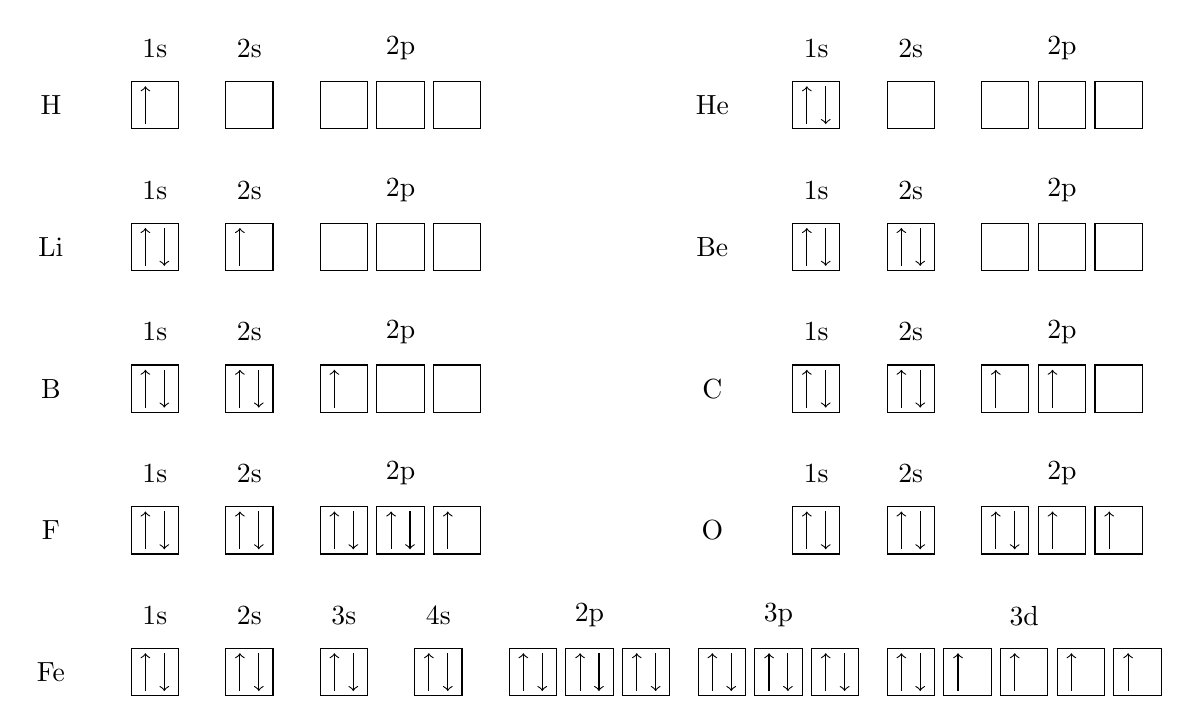
\begin{tikzpicture}[scale=1.2]
    \begin{scope}[shift={(0,-1.5)}]
        \node at (-1,0) {$\mathrm{F}$};

        \node at (0.1,0.6) {1s};
        \node at (1.1,0.6) {2s};
        \node at (2.7,0.6) {2p};
        
        \draw[->] (0,-0.2) -- (0,0.2);
        \draw[->] (0.2,0.2) -- (0.2,-0.2);
        \draw ( -0.15, -0.25) rectangle (0.35,0.25);
        
        \draw[->] (1,-0.2) -- (1,0.2);
        \draw[->] (1.2,0.2) -- (1.2,-0.2);
        \draw (0.85,-0.25) rectangle (1.35,0.25);
        
        \draw[->] (2,-0.2) -- (2,0.2);
        \draw[->] (2.2,0.2) -- (2.2,-0.2);
        \draw (1.85,-0.25) rectangle (2.35,0.25);
        
        \draw[->] (2.6,-0.2) -- (2.6,0.2);
        \draw[->] (2.8,0.2) -- (2.8,-0.2);
        \draw (2.45,-0.25) rectangle (2.95,0.25);
        
        \draw[->] (3.2,-0.2) -- (3.2,0.2);
        \draw (3.05,-0.25) rectangle (3.55,0.25);
    \end{scope}

    \begin{scope}[shift={(7,-1.5)}]
        \node at (-1,0) {$\mathrm{O}$};

        \node at (0.1,0.6) {1s};
        \node at (1.1,0.6) {2s};
        \node at (2.7,0.6) {2p};
        
        \draw[->] (0,-0.2) -- (0,0.2);
        \draw[->] (0.2,0.2) -- (0.2,-0.2);
        \draw ( -0.15, -0.25) rectangle (0.35,0.25);
        
        \draw[->] (1,-0.2) -- (1,0.2);
        \draw[->] (1.2,0.2) -- (1.2,-0.2);
        \draw (0.85,-0.25) rectangle (1.35,0.25);
        
        \draw[->] (2,-0.2) -- (2,0.2);
        \draw[->] (2.2,0.2) -- (2.2,-0.2);
        \draw (1.85,-0.25) rectangle (2.35,0.25);
        
        \draw[->] (2.6,-0.2) -- (2.6,0.2);
        \draw (2.45,-0.25) rectangle (2.95,0.25);
        
        \draw[->] (3.2,-0.2) -- (3.2,0.2);
        \draw (3.05,-0.25) rectangle (3.55,0.25);
    \end{scope}

    \begin{scope}[shift={(0,0)}]
        \node at (-1,0) {$\mathrm{B}$};

        \node at (0.1,0.6) {1s};
        \node at (1.1,0.6) {2s};
        \node at (2.7,0.6) {2p};
        
        \draw[->] (0,-0.2) -- (0,0.2);
        \draw[->] (0.2,0.2) -- (0.2,-0.2);
        \draw ( -0.15, -0.25) rectangle (0.35,0.25);
        
        \draw[->] (1,-0.2) -- (1,0.2);
        \draw[->] (1.2,0.2) -- (1.2,-0.2);
        \draw (0.85,-0.25) rectangle (1.35,0.25);
        
        \draw[->] (2,-0.2) -- (2,0.2);
        \draw (1.85,-0.25) rectangle (2.35,0.25);
        
        \draw (2.45,-0.25) rectangle (2.95,0.25);
        
        \draw (3.05,-0.25) rectangle (3.55,0.25);
    \end{scope}

    \begin{scope}[shift={(7,0)}]
        \node at (-1,0) {$\mathrm{C}$};

        \node at (0.1,0.6) {1s};
        \node at (1.1,0.6) {2s};
        \node at (2.7,0.6) {2p};
        
        \draw[->] (0,-0.2) -- (0,0.2);
        \draw[->] (0.2,0.2) -- (0.2,-0.2);
        \draw ( -0.15, -0.25) rectangle (0.35,0.25);
        
        \draw[->] (1,-0.2) -- (1,0.2);
        \draw[->] (1.2,0.2) -- (1.2,-0.2);
        \draw (0.85,-0.25) rectangle (1.35,0.25);
        
        \draw[->] (2,-0.2) -- (2,0.2);
        \draw (1.85,-0.25) rectangle (2.35,0.25);
        
        \draw[->] (2.6,-0.2) -- (2.6,0.2);
        \draw (2.45,-0.25) rectangle (2.95,0.25);

        \draw (3.05,-0.25) rectangle (3.55,0.25);
    \end{scope}

    \begin{scope}[shift={(0,3)}]
        \node at (-1,0) {$\mathrm{H}$};

        \node at (0.1,0.6) {1s};
        \node at (1.1,0.6) {2s};
        \node at (2.7,0.6) {2p};
        
        \draw[->] (0,-0.2) -- (0,0.2);
        \draw ( -0.15, -0.25) rectangle (0.35,0.25);
        
        \draw (0.85,-0.25) rectangle (1.35,0.25);
        
        \draw (1.85,-0.25) rectangle (2.35,0.25);
        
        \draw (2.45,-0.25) rectangle (2.95,0.25);
        
        \draw (3.05,-0.25) rectangle (3.55,0.25);
    \end{scope}

    \begin{scope}[shift={(7,3)}]
        \node at (-1,0) {$\mathrm{He}$};

        \node at (0.1,0.6) {1s};
        \node at (1.1,0.6) {2s};
        \node at (2.7,0.6) {2p};
        
        \draw[->] (0,-0.2) -- (0,0.2);
        \draw[->] (0.2,0.2) -- (0.2,-0.2);
        \draw ( -0.15, -0.25) rectangle (0.35,0.25);
        
        \draw (0.85,-0.25) rectangle (1.35,0.25);
        
        \draw (1.85,-0.25) rectangle (2.35,0.25);
        
        \draw (2.45,-0.25) rectangle (2.95,0.25);
        
        \draw (3.05,-0.25) rectangle (3.55,0.25);
    \end{scope}

    \begin{scope}[shift={(0,1.5)}]
        \node at (-1,0) {$\mathrm{Li}$};

        \node at (0.1,0.6) {1s};
        \node at (1.1,0.6) {2s};
        \node at (2.7,0.6) {2p};
        
        \draw[->] (0,-0.2) -- (0,0.2);
        \draw[->] (0.2,0.2) -- (0.2,-0.2);
        \draw ( -0.15, -0.25) rectangle (0.35,0.25);
        
        \draw[->] (1,-0.2) -- (1,0.2);
        \draw (0.85,-0.25) rectangle (1.35,0.25);
        
        \draw (1.85,-0.25) rectangle (2.35,0.25);
        
        \draw (2.45,-0.25) rectangle (2.95,0.25);
        
        \draw (3.05,-0.25) rectangle (3.55,0.25);
    \end{scope}

    \begin{scope}[shift={(7,1.5)}]
        \node at (-1,0) {$\mathrm{Be}$};

        \node at (0.1,0.6) {1s};
        \node at (1.1,0.6) {2s};
        \node at (2.7,0.6) {2p};
        
        \draw[->] (0,-0.2) -- (0,0.2);
        \draw[->] (0.2,0.2) -- (0.2,-0.2);
        \draw ( -0.15, -0.25) rectangle (0.35,0.25);
        
        \draw[->] (1,-0.2) -- (1,0.2);
        \draw[->] (1.2,0.2) -- (1.2,-0.2);
        \draw (0.85,-0.25) rectangle (1.35,0.25);
        
        \draw (1.85,-0.25) rectangle (2.35,0.25);
        
        \draw (2.45,-0.25) rectangle (2.95,0.25);
        
        \draw (3.05,-0.25) rectangle (3.55,0.25);
    \end{scope}

    \begin{scope}[shift={(0,-3)}]
        \node at (-1,0) {$\mathrm{Fe}$};

        \node at (0.1,0.6) {1s};
        
        \draw[->] (0,-0.2) -- (0,0.2);
        \draw[->] (0.2,0.2) -- (0.2,-0.2);
        \draw ( -0.15, -0.25) rectangle (0.35,0.25);
        
        \node at (1.1,0.6) {2s};
        \draw[->] (1,-0.2) -- (1,0.2);
        \draw[->] (1.2,0.2) -- (1.2,-0.2);
        \draw (0.85,-0.25) rectangle (1.35,0.25);
        
        \node at (2.1,0.6) {3s};
        \draw[->] (2,-0.2) -- (2,0.2);
        \draw[->] (2.2,0.2) -- (2.2,-0.2);
        \draw (1.85,-0.25) rectangle (2.35,0.25);
        
        \node at (3.1,0.6) {4s};
        \draw[->] (3,-0.2) -- (3,0.2);
        \draw[->] (3.2,0.2) -- (3.2,-0.2);
        \draw (2.85,-0.25) rectangle (3.35,0.25);
        
        \node at (4.7,0.6) {2p};

        \draw[->] (4,-0.2) -- (4,0.2);
        \draw[->] (4.2,0.2) -- (4.2,-0.2);
        \draw (3.85,-0.25) rectangle (4.35,0.25);
        
        \draw[->] (4.6,-0.2) -- (4.6,0.2);
        \draw[->] (4.8,0.2) -- (4.8,-0.2);
        \draw (4.45,-0.25) rectangle (4.95,0.25);
        
        \draw[->] (5.2,-0.2) -- (5.2,0.2);
        \draw[->] (5.4,0.2) -- (5.4,-0.2);
        \draw (5.05,-0.25) rectangle (5.55,0.25);
        
        \node at (6.7,0.6) {3p};

        \draw[->] (6,-0.2) -- (6,0.2);
        \draw[->] (6.2,0.2) -- (6.2,-0.2);
        \draw (5.85,-0.25) rectangle (6.35,0.25);
        
        \draw[->] (6.6,-0.2) -- (6.6,0.2);
        \draw[->] (6.8,0.2) -- (6.8,-0.2);
        \draw (6.45,-0.25) rectangle (6.95,0.25);
        
        \draw[->] (7.2,-0.2) -- (7.2,0.2);
        \draw[->] (7.4,0.2) -- (7.4,-0.2);
        \draw (7.05,-0.25) rectangle (7.55,0.25);
        
        \node at (9.3,0.6) {3d};

        \draw[->] (8,-0.2) -- (8,0.2);
        \draw[->] (8.2,0.2) -- (8.2,-0.2);
        \draw (7.85,-0.25) rectangle (8.35,0.25);
        
        \draw[->] (8.6,-0.2) -- (8.6,0.2);
        \draw (8.45,-0.25) rectangle (8.95,0.25);
        
        \draw[->] (9.2,-0.2) -- (9.2,0.2);
        \draw (9.05,-0.25) rectangle (9.55,0.25);
        
        \draw[->] (9.8,-0.2) -- (9.8,0.2);
        \draw (9.65,-0.25) rectangle (10.15,0.25);
        
        \draw[->] (10.4,-0.2) -- (10.4,0.2);
        \draw (10.25,-0.25) rectangle (10.75,0.25);
    \end{scope}

\end{tikzpicture}
\end{center}

Здесь у гелия 2 электрона на первой s-орбитали, поэтому электронная конфигурация записывается как $1\text{s}^2$. Для железа электронная конфигурация записывается как $1\text{s}^2\ 2\text{s}^2\ 2\text{p}^6\ 3\text{s}^2\ 3\text{p}^6\ 4\text{s}^2\ 3\text{d}^6$

\mediumvspace

Полный момент электрона складывается из орбитального момента $\vec L$ и спинового момента $\vec S$, и называется полным моментом $\vec J = \vec L + \vec S$. Его величина равна

\[
J = \sqrt{j(j+1)} \hbar, \quad j = |l-s|, \dots, l+s.
\]

Когда внутренняя оболочка не заполнена, а заполняется внешняя, электроны имеют несбалансированные спины и орбитальные моменты. Это приводит к образованию так называемых магнитных моментов, из которых складываются макроскопические магнитные свойства вещества. Именно такие элементы, как железо, кобальт и никель, становятся сильными магнитами

\smallvspace

Число квантово-доступных состояний на одном энергетическом уровне определяется формулой $2 n^2$, где $n$ — главное квантовое число. Это учитывает все возможные значения $l$, $m$ и спин $s = \frac12$ для электрона

\smallvspace

Энергетические уровни в атоме могут расщепляться из-за взаимодействий спина и орбитального момента (спин-орбитальное взаимодействие) или из-за внешнего магнитного поля, как в опыте Зеемана. Зееман помещал пламя, в котором были распылены натриевые соли, между полюсами очень сильного магнита. Затем он наблюдал спектр излучения через спектроскоп. Ожидалось, что спектр не изменится -- ведь классическая физика тогда не предсказывала влияния магнетизма на частоты света

Но Зееман заметил, что спектральные линии начали расширяться, а при усилении поля линия раздробилась на несколько компонент. Это стало первым прямым доказательством того, что атомы имеют магнитный момент, а энергетические уровни расщепляются в магнитном поле

\smallvspace

Некоторые переходы между энергетическими уровнями запрещены законом квантовой механики. Например:
\begin{itemize}
    \item Переходы, не удовлетворяющие правилу отбора $\Delta l = \pm 1$ (для орбитального квантового числа)
    \item Переходы, не удовлетворяющие изменению проекции магнитного числа $\Delta m = 0, \pm 1$
    \item Переходы, при которых спин электрона меняется (спин-неразрешённые переходы)
\end{itemize}

Такие запреты определяют спектральные линии атомов, их интенсивность и возможность использования в лазерах, спектроскопии и квантовой электронике
